\section{Evaluation metrics}

This section describes the metrics used to evaluate depth, ego motion, feature point and consensus maximization predictions. These specific metrics where chosen because they are also used in the related works in this field, which makes the results comparable to other papers.

\subsection{Depth error and accuracy metrics}
\label{sec:depthmetrics}

The depth error and accuracy metrics are sparse and only calculated for the pixels of which there exists a ground truth laser measurement in the dataset. The values are averaged over all laser measurements and frames in the test split of the dataset. An error of 0 and an accuracy of 1 is optimal, but can never be achieved in practice.

The depth is predicted relative to an unknown scale, and the ground truth is measured in meters. To alleviate this issue the depth predictions are scaled so that their median is the same as the median of the ground truth for each frame. This does not guarantee that the unit of the predictions is meters, but at least it makes the scales somewhat similar.

The error metrics used in the results chapter are referred to as \textit{Abs Rel}, \textit{Sq Rel}, \textit{RMSE} and \textit{RMSLE}.

The \textit{Abs Rel} error is based on \textit{MAE} which is the mean of the absolute errors which means that it has the same unit as the errors, and is conceptually quite easy to interpret.

\[
\textrm{MAE}=\frac{\sum^N_{n=1}{|y_n-\hat{y}_n|}}{N}
\]

Because the depth from the neural network is without unit and only predicted relative to an unknown scale, a variation on the \textit{MSE} metric called \textit{Abs Rel} is used.

\[
\textrm{Abs Rel}=\frac{\sum^N_{n=1}{\frac{|y_n-\hat{y}_n|}{y_n}}}{N}
\]

The \textit{MSE} metric is the mean of squared errors, for an unbiased estimator it represents the variance of the errors. 

\[
\textrm{MSE}=\frac{\sum^N_{n=1}{(y_n-\hat{y}_n)^2}}{N}
\]

Once again, because the depth is predicted relative to an unknown scale a variation on \textit{MSE} called \textit{Sq Rel} is used instead.

\[
\textrm{Sq Rel}=\frac{\sum^N_{n=1}{\frac{(y_n-\hat{y}_n)^2}{y_n}}}{N}
\]

The \textit{RMSE} metric is the square root of the mean of squared errors. For an unbiased estimator it represents the standard deviation of the errors. Because the errors are squared in the \textit{RMSE} metric it is more sensitive to outliers that for example \textit{MSE}.

\[
\textrm{RMSE}=\sqrt{\frac{\sum^N_{n=1}{(y_n-\hat{y}_n)^2}}{N}}
\]

The \textit{RMSLE} metric is similar to \textit{RMSE} but is useful because it penalizes large errors less when both the actual and predicted values are large.

\[
\textrm{RMSLE}=\sqrt{\frac{\sum^N_{n=1}{(\log{y_n}-\log{\hat{y}_n)}^2}}{N}}
\]

To measure the depth accuracy, in the range from 0 to 1, the following metric is used.

\[
a_{\gamma} = \frac{\sum^N_{n=1}{(\max(\frac{y_n}{\hat{y}_n}, \frac{\hat{y}_n}{y_n}) < \gamma)}}{N},\textrm{ for }\gamma \in \{1.25, 1.25^2, 1.25^3\}
\]

This should be interpreted as the ratio of predictions that is within the ratio of $ \gamma $ relative to the ground truth.

\subsection{Camera ego motion error metric}
\label{sec:egometric}

The error of the camera motion predictions are measured using \textit{RMSE}. But instead of taking the mean error over all poses in a sequence, the alignment error is calculated part wise over a track length of only 5 poses. The final error is presented as the mean \textit{RMSE} of all parts. Each track part from the prediction is transformed to have its first pose coincide with the ground truth in a common origo. This is done so that the first pose in the track part of both the prediction and ground truth is the identity matrix $I \in \mathbb{R}^{4\times 4}$. Because the ego motion is predicted relative to an unknown scale and the ground truth is in meters, we scale each predicted track part to have similar scale to the ground truth track part.

\subsection{Keypoint error and score metrics}\label{sec:keypointmetrics}

The unsupervised keypoint network was compared with the ORB feature detector from OpenCV. To messure the performance differences 3 different metrics where used, repeatability score (RS), localization error (LE), matching score (MS), and matching ratio (MR).

Before any of the metrics are calculated the points are first filtered to remove all points within 10px of the edges. This is done to not include detections where the black background meets the border of the transformed image.

\begin{figure}[H]
	\centering
	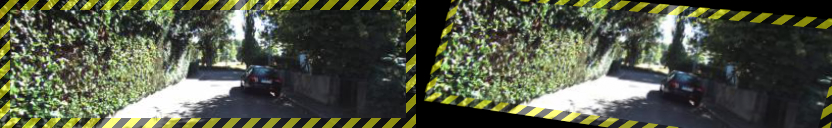
\includegraphics[width=1.0\textwidth]{remove-edges}
	\caption{The black and yellow stripes illustrates the are where keypoint detections are filtered out and discarded.}
	\label{fig:remove-edges}
\end{figure}

To calculate the set of ground truth correspondences, the points in the left image is transformed by the known homography $H$. A point in the left image is corresponding with a point in the right image if they are their closes neighbor and the distance is less than 3px after the transformation. This set of ground truth correspondences is used in all metrics. If the images contain a different amount of points, the largest set of possible correspondences that could have been found is $N_{tot} = \min(N_{left}, N_{right})$. The number of ground truth correspondences (closer than 3px) is $N_{gt} \le N_{tot}$.

Repeatability score (RS) is a measure on how good a method is at repeatedly highlighting the same physical features in the scene but in different images. Because the keypoint algorithm is only fed one image at the time, it is important that there is consistency in what physical features are selected in the image, otherwise their will be very few actual correspondences.

\[
RS = \frac{N_{gt}}{N_{tot}} 
\]

Localization error (LE) is a measure of the average distance error between the ground truth corresponding points. It will always be less than 3px because that is our definition of a correspondence, but the ideal is 0px.


Matching score (MS) is a measure on how many keypoints are matched correctly based on their descriptors. The set of points that are both ground truth correspondences and are corresponding based on their predicted descriptors are said to be correctly matched. The number of correctly matched points are $N_{correct}$.

\[
MS=\frac{N_{correct}}{N_{tot}}
\]

Matching ratio (MR) is very similar to matching score. To get a high MS requires both good repeatability and good descriptors, but getting an MR requires only good descriptors.

\[
MR=\frac{N_{correct}}{N_{gt}}
\]

\subsection{Consensus maximization performance metrics}

The unsupervised consensus maximization network that predicts homographies was compared with the \textit{findHomography()} function in OpenCV.

The homography error (HE) is calculated as the average distance between the corners of the image when it is transformed by the estimated homography compared to the ground truth homography.

\begin{figure}[H]
	\centering
	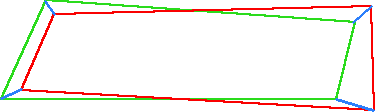
\includegraphics[width=0.5\textwidth]{he}
	\caption{The corners of the image transformed by the ground truth homography and the predicted homography is shown in green and red respectively. The homography error (HE) is calculated as the average of the distances shown in blue.}
	\label{fig:he}
\end{figure}

In order to evaluate the methods ability to distinguish inliers and outliers among the points, a confusion matrix is used. The ground truth set of inliers, or ideal, is the same as the one calculated in section \ref{sec:keypointmetrics}. The confusion matrix shows the ratio of true positives, true negatives, false positives and false negatives in the inlier classifications. The confusion matrix is normalized on the axis of ground truth so that the sum of true positives and false negatives adds up to 1, and the sum of the false positives and true negatives also adds up to one.

\begin{table}[H]
	\centering
	\begin{tabular}{l|l|c|c|c}
		\multicolumn{2}{c}{}&\multicolumn{2}{c}{Predicted}&\\
		\cline{3-4}
		\multicolumn{2}{c|}{}&Inlier&Outlier&\multicolumn{1}{c}{Total}\\
		\cline{2-4}
		\multirow{2}{*}{Actual}& Inlier & TP & FN & $TP+FN=1$\\
		\cline{2-4}
		& Outlier & FP & TN & $FP+TN=1$\\
		\cline{2-4}
		\multicolumn{1}{c}{} & \multicolumn{1}{c}{Total} & \multicolumn{1}{c}{$TP+FP$} & \multicolumn{    1}{c}{$FN+TN$} & \multicolumn{1}{c}{$2$}\\
	\end{tabular}
	\caption{Structure of confusion matrix for inlier classification.}
	\label{table:confusion}
\end{table}
